\documentclass{standalone}
\usepackage{tikz}
\begin{document}
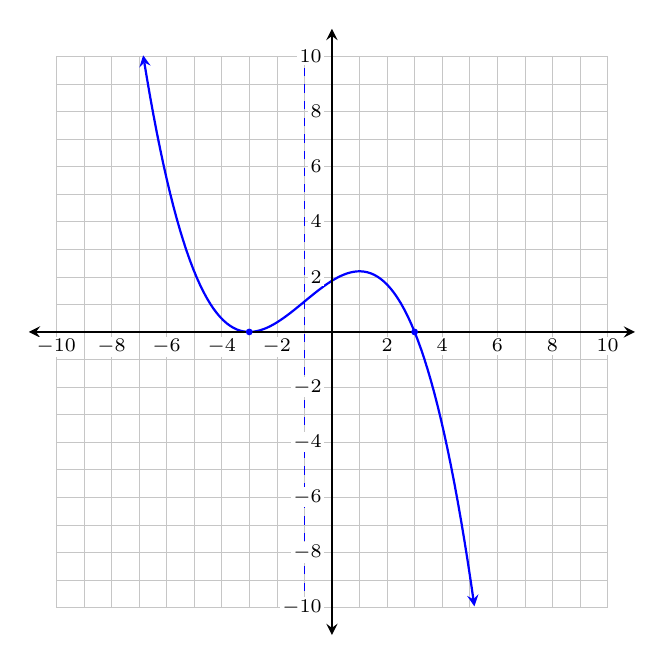
\begin{tikzpicture}[>=stealth, scale=0.35]
  % Same blank grid as 10B, with a sample answer graph drawn on it
  \draw[gray!45, very thin] (-10,-10) grid (10,10);
  % Cubic f(x) = -0.06875 (x+3)^2 (x-3): zeros at x = -3 and x = 3,
  % inflection at x = -1, so it is concave up left of -1 and concave
  % down right of it. Domain runs from f(x) = 10 to f(x) = -10.
  \draw[<->, thick, blue] plot[domain=-6.85:5.17, samples=100]
    (\x, {-0.06875*(\x+3)^2*(\x-3)});
  % Inflection point marked with a dashed vertical line at x = -1
  \draw[blue, dashed] (-1,-10) -- (-1,10);
  % Axes and labels drawn last so they sit on top of the curve
  \draw[<->, thick] (-11,0) -- (11,0);
  \draw[<->, thick] (0,-11) -- (0,11);
  \foreach \x in {-10,-8,-6,-4,-2,2,4,6,8,10} {
    \node[below, font=\scriptsize, fill=white, inner sep=1pt] at (\x,-0.15) {$\x$};
  }
  \foreach \y in {-10,-8,-6,-4,-2,2,4,6,8,10} {
    \node[left, font=\scriptsize, fill=white, inner sep=1pt] at (-0.25,\y) {$\y$};
  }
  % The two zeros highlighted
  \fill[blue] (-3,0) circle (3.5pt);
  \fill[blue] (3,0) circle (3.5pt);
\end{tikzpicture}
\end{document}
